\documentclass[stochastic-or.tex]{subfiles}
\usepackage{amsmath} % this is only used to enforce good environment completion in emacs
\externaldocument{stochastic-or}

\loadgeometry{tufte}

\begin{document}

\section{Renewal Reward Theorem}
\label{sec:renew-reward-theor}

In a one-dollar store, each item costs $\$ 1$.
If every minute a customer arrives, and each customer buys exactly $10$ items, this shop earns money at a rate of $ \$ 10$ per minute.
At another shop, customers spend variable amounts but on average $\$ 10$ per customer, and customers come in irregularly, but the average inter-arrival time between two customers is~$1$ minute.
This other shop also earns money at rate of $\$ 10$ per minute.
That both shops have the same earning rate is what the \recall{renewal reward} theorem says.
In this section we prove this extremely useful theorem and show how to apply it to queueing and inventory systems.


\newthought{We are given} a sequence of strictly increasing epochs $0=T_0 < T_1 < T_2 < \cdots$ such that $T_k\to\infty$ as $k\to\infty$, and a non-decreasing right-continuous (deterministic) function $t\to Y(t)$ with $Y(0)=0$.
Let $N(t) = \sum_{k=1}^{\infty} \1{T_k\leq t}$ count the number of epochs that occurred during $(0, t]$, and $X_k = Y(T_k)-Y(T_{k-1})$ be the increment of $Y(t)$ during $(T_{k-1}, T_{k}]$.\sidenote{Here $X_k$ is not necessary an inter-arrival time between two jobs.}
\cref{fig:renewal} shows graphically how all concepts relate.



\begin{theorem}[Renewal Reward Theorem, $Y=\lambda X$]
Assume  that the limit $\lambda=\lim_{t\to\infty}N(t)/t$ exists with $0<\lambda<\infty$.
Then, the limit $Y=\lim_{t\to\infty}Y(t)/t$ exists iff $X = \lim_{n\to\infty} n^{-1}\sum_{k=1}^{n}X_{k}$ exists, in which
 case, $Y=\lambda X$.
\end{theorem}

\begin{proof}
To see why this is true, we copy an idea of~\cref{sec:rate-stability}. Just as with the relation between $A(t)$ and $A_{A(t)}$, we have here that  $T_{N(t)} \leq t < T_{N(t)+1}$. As $Y(\cdot)$ is non-decreasing,
\begin{equation*}
  Y(T_{N(t)}) \leq Y(t) \leq Y(T_{N(t)+1}),
\end{equation*}
hence
\begin{align*}
\frac{N(t)}{t} \frac{Y(T_{N(t)})}{N(t)}  &\leq \frac{Y(t)} t \leq \frac{Y(T_{N(t)+1})}{N(t)+1} \frac{N(t)+1}{t}.
\end{align*}
Noting that $Y(T_{N(t)}) = \sum_{k=1}^{N(t)} X_{k}$, and using the assumption that $N(t)/t \to \lambda$ we conclude that $Y(t)/t \to Y$ iff $(N(t))^{-1}\sum_{k=1}^{N(t)} X_{k} \to X$.
If one of these limits exists, the other exists, hence $Y=\lambda X$.
\end{proof}




\begin{figure}[t]
 \centering
 \begin{tabular}{cc}
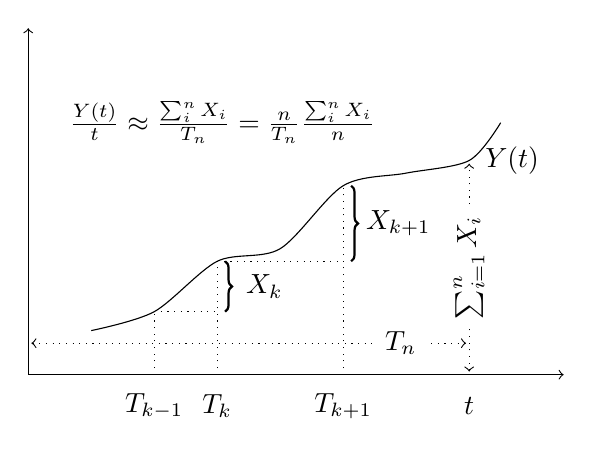
\begin{tikzpicture}[scale=0.8]
%axis
\draw[->] (0,0) -- coordinate (x axis mid) (8.5,0);
\draw[->] (0,0) -- coordinate (y axis mid) (0,5.5);
%\node[below=0.2cm] at (x axis mid) {$t$};

\draw plot [smooth] coordinates {(1,0.7) (2,1) (3,1.8) (4,2) (5,3) (6,3.2) (7, 3.4) (7.5,4.0)};
\node[right] at (7.1,3.4) {$Y(t)$};
\node at (7.,-0.5) {$t$};

\node at (2.,-0.5) {$T_{k-1}$};
\draw[dotted] (2,0)--(2,1);
\draw[dotted] (2,1)--(3,1);


\node at (3.,-0.5) {$T_{k}$};
\draw[dotted] (3,0)--(3,1.8);
\draw[dotted] (3,1.8)--(5,1.8);

\draw [
 thick,
 decoration={brace, mirror, raise=0.1cm },
 decorate
] (3,1) -- (3,1.8)
node[pos=0.5, xshift=0.6cm] {$X_k$};


\node at (5.,-0.5) {$T_{k+1}$};
\draw[dotted] (5,0)--(5,3);

\draw [
 thick,
 decoration={brace, mirror, raise=0.1cm },
 decorate
] (5,1.8) -- (5,3)
node[pos=0.5, xshift=0.7cm] {$X_{k+1}$};

\node[right] at (0.5,4) {$\frac{Y(t)}t \approx \frac{\sum_i^n X_i}{T_n} = \frac{n}{T_n} \frac{\sum_i^n X_i}n $};


\draw[dotted,<->, =stealth] (7,0.05)--(7,3.35) node[midway, rotate=90, fill=white] {$\sum_{i=1}^n X_i$};
\draw[dotted,<->, =stealth] (0.05,0.5)--(6.95,0.5) node[pos=0.85, fill=white] {$T_n$};
\end{tikzpicture}
&
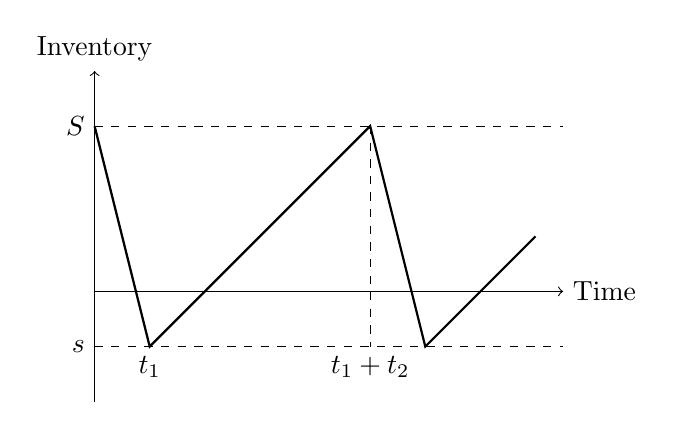
\begin{tikzpicture}[scale=0.7]
\draw[->] (0,0) -- (8.5,0) node[right] {Time};
\draw[->] (0,-2) -- (0,4) node[above] {Inventory};

\draw[] (0,3) node[left] {$S$} ;
\draw[dashed] (0,3) -- (8.5,3);
\draw[] (0,-1) node[left] {$s$};
\draw[dashed] (0,-1) -- (8.5,-1);
\draw[color=black, thick] (0, 3)--(1, -1)--(5,3)--(6, -1)--(8, 1);
\draw[] (1, -1) node[below] {$t_1$};

\draw[dashed] (5,3) -- (5,-1);
\draw[] (5, -1) node[below] {$t_1+t_2$};
\end{tikzpicture}
 \end{tabular}
 \caption{The left panel provides a graphical `proof' of the renewal reward equation $Y=\lambda X$.
The right panel shows a sample path of an inventory system with constant production capacity and a fixed demand rate.
As the inventory is operated under an $(s,S)$-policy, it is a system that moves from cycle to cycle.}
\label{fig:renewal}
\end{figure}



\newthought{The renewal reward} theorem finds an easy application in the analysis of the \recall{Economic Production Quantity} (EPQ) model which is an inventory system in which demand arrives at a fixed rate~$d$ and items are produced at constant rate~$r$ by a machine that can switch on and off.\sidenote{The EOP model is a production-inventory system with a constant demand rate.}
The inventory is under an $(s,S)$ policy, the leadtime $L=0$, the holding and backlogging cost are~$h$ and~$b$ per unit per time, and it costs~$K$ to switch on the machine.
\cref{fig:renewal} shows a sample path of the inventory level.
Let us use the ideas of renewal reward theory to find the policy parameters that minimize the long-run time average cost.


Clearly, the inventory level repeats over time, so it suffices to study just one cycle that starts and stops when the inventory level hits~$S$.
From~\cref{fig:renewal} it is simple to see that
  \begin{align*}
    t_1 &= \frac{S-s}{d}, & t_2 &= \frac{S-s}{r-d}, & T = t_1+t_{2} = \frac{S-s}{d}\frac{r}{r-d},
  \end{align*}
are the time to empty the inventory from level~$S$ to~$s$ (after which production switches on) and the time needed to replenish the inventory from level~$s$ to~$S$ (after which production switches off).

Let us next assume that $s\leq 0 < S$. Then, writing $T_+$ ($T_-$) for the amount of time that the inventory is positive (negative) during a cycle, it follows that
\begin{align*}
\frac{T_+}T &= \frac{S}{S-s},
& \frac{T_-}T &= \frac{-s}{S-s}.
\end{align*}
Using that the holding and backlogging cost are proportional to the areas of the related triangles,  the average cost of one cycle becomes\sidenote{When $0\leq s < S$, $g=K/T + h(s+S)/2$, and when $s<S \leq 0$, $g=K/T + b|s+S|/2$.}
\begin{align*}
g &=\frac{K}{T} +  b\frac{-s}{2} \frac{T_-} T  + h\frac{S}{2} \frac{T_+}{T}.
\end{align*}
Substituting the expressions for $T_{-}, T_{+}$, and $T$ in terms of~$s$ and~$S$, taking the partial derivatives with respect to~$s$ and~$S$ and solving for the optimal values by setting $\partial g/\partial s = \partial g/\partial S = 0$ gives
\begin{align}\label{eq:renewal1}
g^{*} &= \sqrt{2Kd} \sqrt{\frac{hb}{h+b}}\sqrt{1-\frac d r}, & s^{*} &= -\frac{g^{*}}b, & S^{*} = \frac{g^{*}}{h}.
\end{align}
Of course we need  $r\geq d$ for stability. Interestingly, when $r=d$, the cost $g^{*} = 0$.\sidenote{Why is that so?}



The (perhaps) most important formula for practical inventory management is the Economic Order Quantity (EOQ) which follows from~\cref{eq:renewal1} by taking $r\to \infty$ and $b\to\infty$, which amount to saying that replenishments arrive immediately and backlogging is not allowed.
This results in
\begin{align*}
g^{*}_{EOQ} &= \sqrt{2Kdh} & s^{*} &= 0, & Q^{*} = \sqrt{\frac{2Kd}{h}},
\end{align*}
where we write $Q^{*}$  instead of $S^{*}$ to indicate that we order in fixed quantities.
Note that the cost in these limits \emph{increases}.\sidenote{Because we add binding constraints to the optimization problem.}
Observe also that the policy that orders the EOQ is an $(s,S)$-policy, a $(Q,r)$-policy, and a $(T,S)$-policy.\sidenote{Recall the policies of~\cref{sec:single-item-invent}.}

An interesting extension is to consider a system which has  constraints on cycle length and order size. Can you find an optimal policy?


% \begin{exercise}\label{ex:l-162}
% Use the renewal reward theorem to prove \cref{eq:49}.
% \begin{solution}
%  It is evident that $X_k = Y(D_k)-Y(D_{k-1})=S_k$, hence $X = \lim_{n\to\infty} n^{-1}\sum_{k=1}^n X_k = \E S$.
% % Also $\lim_{t\to\infty} Y(t)/t=\rho$.
%  In the relation $Y = \lambda X$, the $\lambda$ is $\delta$ since we consider departure epochs $T_k = D_k$, rather than $A_k$.
%  Thus, with the renewal reward theorem $Y=\lambda X$, we get that $Y = \lim_{t\to\infty} t^{-1} \int_0^t \1{\L(s)>0} \d s = \delta \E S$.
% Observe that the~$Y$ is the long-run fraction of time the server is busy.
% \end{solution}
% \end{exercise}

\begin{truefalse}
Consider a machine which fails regularly and needs to be repaired.
Assuming the repairs take a negligible amount of time, the time between machine failures has density $f_X$, and each repair costs $c$.
Claim, then renewal reward theory inform us that: $\text{cost rate} = \frac{c}{\int_{0}^{\infty} x f(x) \d x}$.
    \begin{solution}
        True. The cost increment per failure is $c$. Thus, this $c$ takes the role of the $X$ in the renewal reward theorem. The time between the failures is $\lambda= 1/\E X$, where $X$ is the (common) interarrival time between two failures. Therefore $Y = c \lambda = c/ \E X$.
    \end{solution}
\end{truefalse}

\begin{truefalse}
Claim:  For the $G/G/1$ queue, if $\E U$ is the expected busy time and
 $\E I$ is the expected idle time, then
\begin{equation*}
\rho =  \E U / (\E U +\E I).
\end{equation*}
\begin{solution} True. See~\cref{ex:57}.
\end{solution}
\end{truefalse}

\begin{truefalse}
Claim.
The following argument proves that $\lambda=\frac{1}{\mathbb{E}[X]}$ by means of the renewal reward theorem.
Let $Y(t)=t$ and $T_k=A_k$, from this it follows that, $X_k=A_k-A_{k-1}$.
Moreover, $\lim\limits_{t\to\infty}\frac{N(t)}{t}=\lambda$.
As $\lim\limits_{t\to\infty}\frac{Y(t)}{t}=1$ we have that $1=\lambda\mathbb{E}[X]$ proving the result.
    \begin{solution}
        True.
    \end{solution}
\end{truefalse}

\begin{truefalse}
    An $(s,S)$-policy is a restocking policy where $s$ denotes the size of replenishment orders, and $S$ represents the speed at which items are produced.
    \begin{solution}
        False.
    \end{solution}
\end{truefalse}


\begin{exercise}
Use the renewal reward theorem to relate the load $\rho=\lambda \E S$ to the limiting fraction of time the server of a stable $G/G/1$ queue is busy.
\begin{hint}
Observe that $Y(t) = \int_0^t \1{\L(s)>0} \d s$ is the total amount of time the server is busy during $[0,t]$, hence $Y(t)/t$ is the fraction of time busy.
Then take $T_k = D_k$ as the epochs at which to inspect $Y(t)$, and realize that $Y(D_{k}) = \sum_{i=1}^{k} S_{i}$.
\end{hint}
\begin{solution}
Take the hint serious. Then, as $k/T_{k} \to \delta$, it follows from the renewal reward theorem that $Y(t)/t \to \delta \E S$.
By rate-stability, $\delta = \lambda$, so that $\rho=\lambda \E S = \delta \E S = Y$, from which the claim follows.

\end{solution}
\end{exercise}


\begin{exercise}\label{ex:70}
We can also derive the relation between utilization and the fraction of busy time of the server of a $G/G/1$ queue by considering the inequalities
\begin{equation}\label{eq:2a}
 \sum_{k=1}^{A(t)} S_k \geq \int_0^t \1{\L(s)>0} \d s \geq \sum_{k=1}^{D(t)} S_k.
\end{equation}
Explain the above and show that by taking appropriate limits we find $\lambda \E S \geq \rho \geq \delta \E S$.
\begin{hint}
For the direction of the inequalities~\cref{eq:2a}, observe that~$t$ can lie half way a service interval, and $A(t) \geq D(t)$.
Divide by~$t$ in~\cref{eq:2a}. Then for the LHS, multiply by $A(t)/A(t)$ and take appropriate limits. Similar for the RHS but multiply by $D(t)/D(t)$.
\end{hint}
\begin{solution}
  For the LHS, as $A(t)\to \infty$ as $t\to\infty$,
\begin{equation*}
 \lim_{t\to\infty} \frac 1 t\sum_{k=1}^{A(t)} S_k =
 \lim_{t\to\infty} \frac{A(t)}t \frac{1}{A(t)} \sum_{k=1}^{A(t)} S_k =
 \lim_{t\to\infty} \frac{A(t)}t \cdot \lim_{t\to\infty}\frac{1}{A(t)} \sum_{k=1}^{A(t)} S_k = \lambda \E S.
\end{equation*}
Apply similar limits to the RHS.
The limit of the middle term gives the fraction of time the server is busy.
\end{solution}
\end{exercise}

\begin{exercise}\label{ex:57}
Show for the $G/G/1$ queue that $\rho = \E \U / (\E \U + \E I)$ where $\E U$ is the expected busy time and $\E I$ the expected idle time.
(The busy time of a server is the time between starting after an idle time until a new idle time starts.)
\begin{solution}
Take $Y(t) = \int_0^t \1{\Ls(s)=1} \d t$. Then, when $U_{k}$ is the~$k$th busy time and $I_{k}$ the~$k$th idle time, let $X_{k} = U_{k}$ and $T_{k} = U_k + I_{k}$.
Then $Y(t)/ t\to\rho$, $X_k/k \to \E \U$, and $(I_k + \U_k)/k \to \E I + \E U = \lambda^{-1}$, i.e., the inverse of the~$\lambda$ we use in the renewal-reward theorem.
\end{solution}
\end{exercise}


\end{document}

